\section{Numerical Implementation in C++}
\label{sec:implementation}

We have provided a numerical implementation of Gaussian Mixture Models in the C++ language
as part of recent releases of the open source Armadillo C++ linear algebra library~\cite{Armadillo_JOSS_2016}. %,Armadillo_PASC_2017}.
The library is available under the permissive Apache 2.0 license~\cite{Laurent_2008},
and can be obtained from
{\texttt{http://arma.sourceforge.net}}.
%\href{http://arma.sourceforge.net}{http://arma.sourceforge.net}.
To considerably reduce execution time,
the implementation contains multi-threaded versions of the EM and {\it k}-means training algorithms
(as overviewed in Sections~\ref{sec:param_em} and~\ref{sec:param_km}).
Implementation of multi-threading (parallelisation) is achieved with the aid of OpenMP compiler directives~\cite{OpenMP_2007}.
% Parallelisation is achieved through refactoring the original EM and {\it k}-means algorithms
% into a MapReduce-like framework~\cite{MapReduce_2004} and employing OpenMP compiler directives~\cite{OpenMP_2007}.

% TODO: choice for $\Mat{\Sigma}$: full or diagonal.
% effects: fewer free parameters; much simpler matrix inverse; simpler computation of the determinant.
% can still model correlations in data through the use of several gaussians -- ref to old Reynolds paper?

There are two main choices for the type of covariance matrix $\Mat{\Sigma}$: full and diagonal.
% The values on the main diagonal (diagonal elements) are variances for each dimension,
% while the off diagonal elements are the covariances across dimensions.
While full covariance matrices have more capacity for modelling data,
diagonal covariance matrices provide several practical advantages:
%
\begin{enumerate}[{\bf (i)}]
\item
the computationally expensive (and potentially unstable) matrix inverse operation in Eqn.~(\ref{eqn:gaussian})
is reduced to simply to taking the reciprocals of the diagonal elements,

\item
the determinant operation is considerably simplified to taking the product of the diagonal elements,

\item
diagonal covariance matrices contain fewer parameters that need to be estimated, and hence require fewer training samples~\cite{Duda01}.
\end{enumerate}

Given the above practical considerations, the implementation uses diagonal covariance matrices.
We note that diagonal covariance GMMs with $N_G > 1$ can model distributions of samples with correlated elements,
which in turn suggests that full covariance GMMs can be approximated using diagonal covariance GMMs with a larger number of Gaussians~\cite{Reynolds_2000}.
% It has also been empirically observed that diagonal covariance GMMs outperform full covariance GMMs~\cite{Reynolds95, Reynolds95b, Reynolds00}.

% In the following text, we first provide a description of the user accessible classes and functions which comprise the implementation,
% followed by a demonstration of the achievable training speedup due to multi-threading.

\subsection{User Accessible Classes and Functions}

The implementation is provided as two user accessible classes within the {\it arma} namespace:
{\small\it gmm\_diag} and~{\small\it fgmm\_diag}.
The former uses double precision floating point values, while the latter uses single precision floating point values.
For an instance of the double precision {\it gmm\_diag} class named as~{\bf M},
its member functions and variables are listed below.
The interface allows the user full control over the parameters for GMM fitting,
as well as easy and flexible access to the trained model.
Figure~\ref{fig:example_usage} contains a complete C++ program which demonstrates usage of the {\it gmm\_diag} class.

In the description below, all vectors and matrices refer to corresponding objects from the Armadillo library;
scalars have the type {\it double},
matrices have the type {\it mat},
column vectors have the type {\it vec},
row vectors have the type {\it rowvec},
row vectors of unsigned integers have the type {\it urowvec},
and indices have the type {\it uword} (representing an unsigned integer).
When using the single precision {\it fgmm\_diag} class,
all vector and matrix types have the {\it f} prefix (for example, {\it fmat}),
while scalars have the type {\it float}.
The word ``heft'' is explicitly used in the classes as a shorter version of ``weight'', while keeping the same meaning with the context of GMMs.


\begin{enumerate}[{$\bullet$}]
\itemsep 1ex

\item
{\bf M.log\_p(V)}\\
return a scalar (double precision floating point value) representing the log-likelihood of column vector {\bf V}

\item
{\bf M.log\_p(V, g)}\\
return a scalar (double precision floating point value) representing the log-likelihood of column vector {\bf V},
according to Gaussian with index~{\bf g} (specified as an unsigned integer of type {\it uword})

\item
{\bf M.log\_p(X)}\\
return a row vector (of type {\it rowvec}) containing log-likelihoods of each column vector in matrix {\bf X}


\item
{\bf M.log\_p(X, g)}\\
return a row vector containing log-likelihoods of each column vector in matrix {\bf X},
according to Gaussian with index {\bf g}  (specified as an unsigned integer of type {\it uword})

\item
{\bf M.avg\_log\_p(X)}\\
return a scalar (double precision floating point value) representing the average log-likelihood of all column vectors in matrix {\bf X}

\item
{\bf M.avg\_log\_p(X, g)}\\
return a scalar (double precision floating point value) representing the average log-likelihood of all column vectors in matrix {\bf X},
according to Gaussian with index~{\bf g}  (specified as an unsigned integer of type {\it uword})

\item
{\bf M.assign(V, dist\_mode)}\\
return an unsigned integer (of type {\it uword}) representing the index of the
closest mean (or Gaussian) to vector {\bf V}; the parameter {\bf dist\_mode} is one
of:
\begin{small}
\begin{enumerate}[{\bf {~eucl\_dist}}]
\item
Euclidean distance (takes only means into account)
\end{enumerate}

\begin{enumerate}[{\bf {prob\_dist}}]
\item
probabilistic ``distance'', defined as the inverse likelihood (takes into account means, covariances and hefts)
\end{enumerate}
\end{small}

% \begin{tabular}{ll}
% {\bf eucl\_dist} & Euclidean distance (takes only means \\
%                  & into account) \\
% {\bf prob\_dist} & probabilistic ``distance'', defined as the \\
%                  & inverse likelihood (takes into account \\
%                  & means, covariances and hefts) \\
% \end{tabular}

\item
{\bf M.assign(X, dist\_mode)}\\
return a row vector of unsigned integers (of type {\it urowvec}) containing the indices of the closest means (or Gaussians) to each column vector in matrix {\bf X};
parameter {\bf dist\_mode} is {\bf eucl\_dist} or {\bf prob\_dist}, as per the {\bf .assign()} function above

\item
{\bf M.raw\_hist(X, dist\_mode)}\\
return a row vector of unsigned integers (of type {\it urowvec}) representing the raw histogram of counts;
each entry is the number of counts corresponding to a Gaussian;
each count is the number times the corresponding Gaussian was the closest to each column vector in matrix {\bf X};
parameter {\bf dist\_mode} is {\bf eucl\_dist} or {\bf prob\_dist}, as per the {\bf .assign()} function above

\item
{\bf M.norm\_hist(X, dist\_mode)}\\
similar to the {\bf .raw\_hist()} function above; return a row vector (of type {\it rowvec}) containing normalised counts; the vector sums to one;
parameter {\bf dist\_mode} is either {\bf eucl\_dist} or {\bf prob\_dist}, as per the {\bf .assign()} function above

\item
{\bf M.generate()}\\
return a column vector representing a random sample generated according to the model's parameters

\item
{\bf M.generate(N)}\\
return a matrix containing {\bf N} column vectors, with each vector representing a random sample generated according to the model's parameters

\item
{\bf M.save(filename)}\\
save the model to a file

\item
{\bf M.load(filename)}\\
load the model from a file

\item
{\bf M.n\_gaus()}\\
return an unsigned integer (of type {\it uword}) containing the number of means/Gaussians in the model

\item
{\bf M.n\_dims()}\\
return an unsigned integer (of type {\it uword}) containing the dimensionality of the means/Gaussians in the model

\item
{\bf M.reset(n\_dims, n\_gaus)}\\
set the model to have dimensionality {\bf n\_dims}, with {\bf n\_gaus} number of Gaussians, specified as unsigned integers of type {\it uword};
all the means are set to zero, all diagonal covariances are set to one, and all the hefts (weights) are set to be uniform

\item
{\bf M.means}\\
read-only matrix (of type {\it mat}) containing the means (centroids), stored as column vectors

\item
{\bf M.dcovs}\\
read-only matrix (of type {\it mat}) containing the diagonal covariances, with the set of diagonal covariances for each Gaussian stored as a column vector

\item
{\bf M.hefts}\\
read-only row vector (of type {\it rowvec}) containing the hefts (weights)

\item
{\bf M.set\_means(X)}\\
set the means (centroids) to be as specified in matrix {\bf X}, with each mean (centroid) stored as a column vector;
the number of means and their dimensionality must match the existing model

\item
{\bf M.set\_dcovs(X)}\\
set the diagonal covariances to be as specified in matrix~{\bf X}, with the set of diagonal covariances for each Gaussian stored as a column vector;
the number of diagonal covariance vectors and their dimensionality must match the existing model

\item
{\bf M.set\_hefts(V)}\\
set the hefts (weights) of the model to be as specified in row vector {\bf V};
the number of hefts must match the existing model

\item
{\bf M.set\_params(means, dcovs, hefts)}\\
set all the parameters at the same time, using matrices denoted as {\bf means} and {\bf dcovs} as well as the row vector denoted as {\bf hefts};
the layout of the matrices is as per the {\bf .set\_means()} and {\bf .set\_dcovs()} functions above;
the number of Gaussians and dimensionality can be different from the existing model

\item
{\bf M.learn(data, n\_gaus, dist\_mode, seed\_mode, km\_iter, em\_iter, var\_floor, print\_mode)}\\
learn the model parameters via the {\it k}-means and/or EM algorithms,
and return a boolean value, with {\it true} indicating success, and {\it false} indicating failure;
the parameters have the following meanings:

\begin{small}
\begin{enumerate}[{-}]
\itemsep 1ex
\item
{\bf data}\\
matrix (of type {\it mat}) containing training samples; each sample is stored as a column vector

\item
{\bf n\_gaus}\\
set the number of Gaussians to {\bf n\_gaus};
to help convergence, it is recommended that the given {\bf data} matrix (above)
contains at least 10 samples for each Gaussian

\item
{\bf dist\_mode}\\
specifies the distance used during the seeding of initial means and {\it k}-means clustering:
\begin{small}
\begin{enumerate}[{\bf eucl\_dist}]
\item Euclidean distance
\end{enumerate}

\begin{enumerate}[{\bf {maha\_dist}}]
\item Mahalanobis distance, which uses a global diagonal covariance matrix estimated from the given training samples
\end{enumerate}
\end{small}

% \begin{tabular}{ll}
% {\bf eucl\_dist} & Euclidean distance\\
% {\bf maha\_dist} & Mahalanobis distance, which uses a \\
%                  & global diagonal covariance matrix \\
%                  & estimated from the given training \\
%                  & samples
% \end{tabular}

\item
{\bf seed\_mode}\\
specifies how the initial means are seeded prior to running {\it k}-means and/or EM algorithms:
\begin{small}
\begin{enumerate}[{\bf {~~~keep\_existing}}]
\item keep the existing model (do not modify the means, covariances and hefts)
\end{enumerate}
\begin{enumerate}[{\bf {~~~~static\_subset}}]
\item a subset of the training samples (repeatable)
\end{enumerate}
\begin{enumerate}[{\bf {~random\_subset}}]
\item a subset of the training samples (random)
\end{enumerate}
\begin{enumerate}[{\bf {~~~static\_spread}}]
\item a maximally spread subset of training samples (repeatable)
\end{enumerate}
\begin{enumerate}[{\bf {random\_spread}}]
\item a maximally spread subset of training samples (random start) \\
\end{enumerate}
\end{small}

% \vspace*{0.5em}
% \begin{tabular}{ll}
% {\bf keep\_existing} & keep the existing model (do not \\
%                      & modify the means, covariances \\
%                      & and hefts) \\
% {\bf static\_subset} & a subset of the training samples \\
%                      & (repeatable) \\
% {\bf random\_subset} & a subset of the training samples \\
%                      & (random) \\
% {\bf static\_spread} & a maximally spread subset of \\
%                      & training samples (repeatable) \\
% {\bf random\_spread} & a maximally spread subset of \\
%                      & training samples (random start) \\
% \end{tabular}
% \vspace*{0.5em}

Note that seeding the initial means with {\bf static\_spread} and {\bf random\_spread}
can be more time consuming than with {\bf static\_subset} and {\bf random\_subset};
these seed modes are inspired by the so-called {\it k-means++} approach~\cite{Arthur_2007}, with the aim to improve clustering quality

\item
{\bf km\_iter}\\
the maximum number of iterations of the {\it k}-means algorithm; this is data dependent, but typically 10 iterations are sufficient

\item
{\bf em\_iter}\\
the maximum number of iterations of the EM algorithm; this is data dependent, but typically 5 to 10 iterations are sufficient

\item
{\bf var\_floor}\\
the variance floor (smallest allowed value) for the diagonal covariances; setting this to a small non-zero value can help with convergence and/or better quality parameter estimates

\item
{\bf print\_mode}\\
boolean value (either {\it true} or {\it false}) which enables/disables the printing of progress during the {\it k}-means and EM algorithms 

\end{enumerate}
\end{small}

\end{enumerate}

% \noindent
% The above interface allows the user full control over the parameters of the GMM
% fitting, and easy access to the trained results.
% In addition, the mlpack machine learning library \cite{Curtin_2013} wraps the {\tt gmm\_diag} class
% to provide a unified frontend for training Gaussian Mixture Models both with diagonal and non-diagonal covariance matrices.

\begin{figure}[!b]
\hrule
\vspace{1ex}
\centering
% possible mono-space fonts: BeraMono, DejaVu Sans Mono, KP Monospaced, LuxiMono, Inconsolata
%\begin{Verbatim}
%\begin{Verbatim}[fontsize=\footnotesize,fontseries=b]
\begin{Verbatim}[fontsize=\footnotesize]
#include <armadillo>

using namespace arma;

int main()
  {
  // create synthetic data containing
  // 2 clusters with normal distribution
  
  uword d = 5;       // dimensionality
  uword N = 10000;   // number of samples (vectors)
  
  mat data(d, N, fill::zeros);
  
  vec mean0 = linspace<vec>(1,d,d);
  vec mean1 = mean0 + 2;
  
  uword i = 0;
  
  while(i < N)
    {
    if(i < N)  { data.col(i) = mean0 + randn<vec>(d); ++i; }
    if(i < N)  { data.col(i) = mean0 + randn<vec>(d); ++i; }
    if(i < N)  { data.col(i) = mean1 + randn<vec>(d); ++i; }
    }
  
  // model the data as a diagonal GMM with 2 Gaussians
  
  gmm_diag model;
  
  bool status = model.learn(data, 2, maha_dist, random_subset,
                            10, 5, 1e-10, true);
  
  if(status == false)  { cout << "learning failed" << endl; }
  
  model.means.print("means:");
  
  double overall_likelihood = model.avg_log_p(data);
  
  rowvec     set_likelihood = model.log_p( data.cols(0,9) );
  double  scalar_likelihood = model.log_p( data.col(0)    );
  
  uword   gaus_id  = model.assign( data.col(0),    eucl_dist );
  urowvec gaus_ids = model.assign( data.cols(0,9), prob_dist );
  
  urowvec hist1 = model.raw_hist (data, prob_dist);
   rowvec hist2 = model.norm_hist(data, eucl_dist);
  
  model.save("my_model.gmm");
  
  return 0;
  }

\end{Verbatim}
\vspace{-1ex}
\hrule
\vspace{0.5ex}
\caption
  {
  An example C++ program which demonstrates usage of several functions from the {\it gmm\_diag} class.
  }
\label{fig:example_usage}
\end{figure}


% Ensure the figure is on the same page as the discussion.
\begin{figure*}[t!]
\centering
\begin{minipage}{\textwidth}
  \centering
  \begin{minipage}{0.5\textwidth}
    \centering
    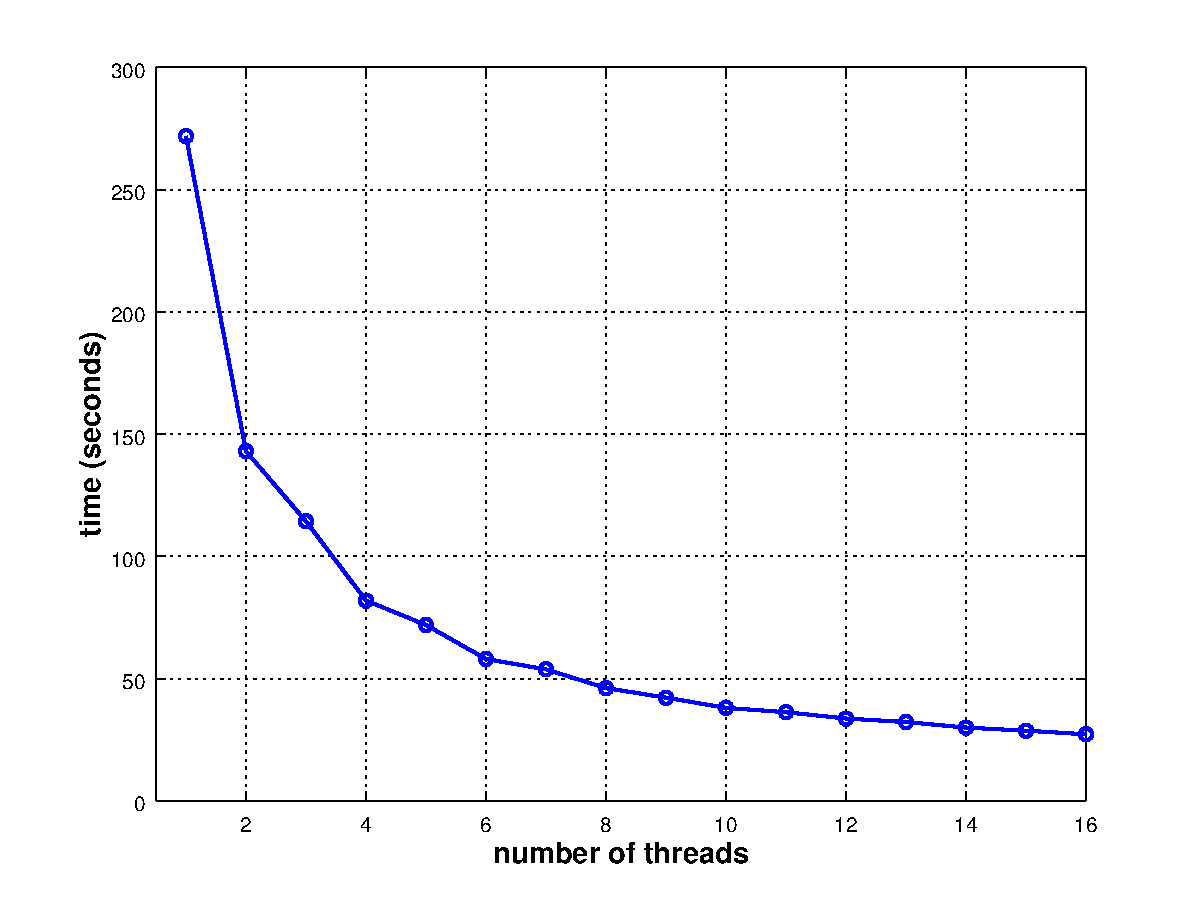
\includegraphics[width=1.1\textwidth]{plot1.pdf}\\
    {(a)}
  \end{minipage}%
  \begin{minipage}{0.5\textwidth}
    \centering
    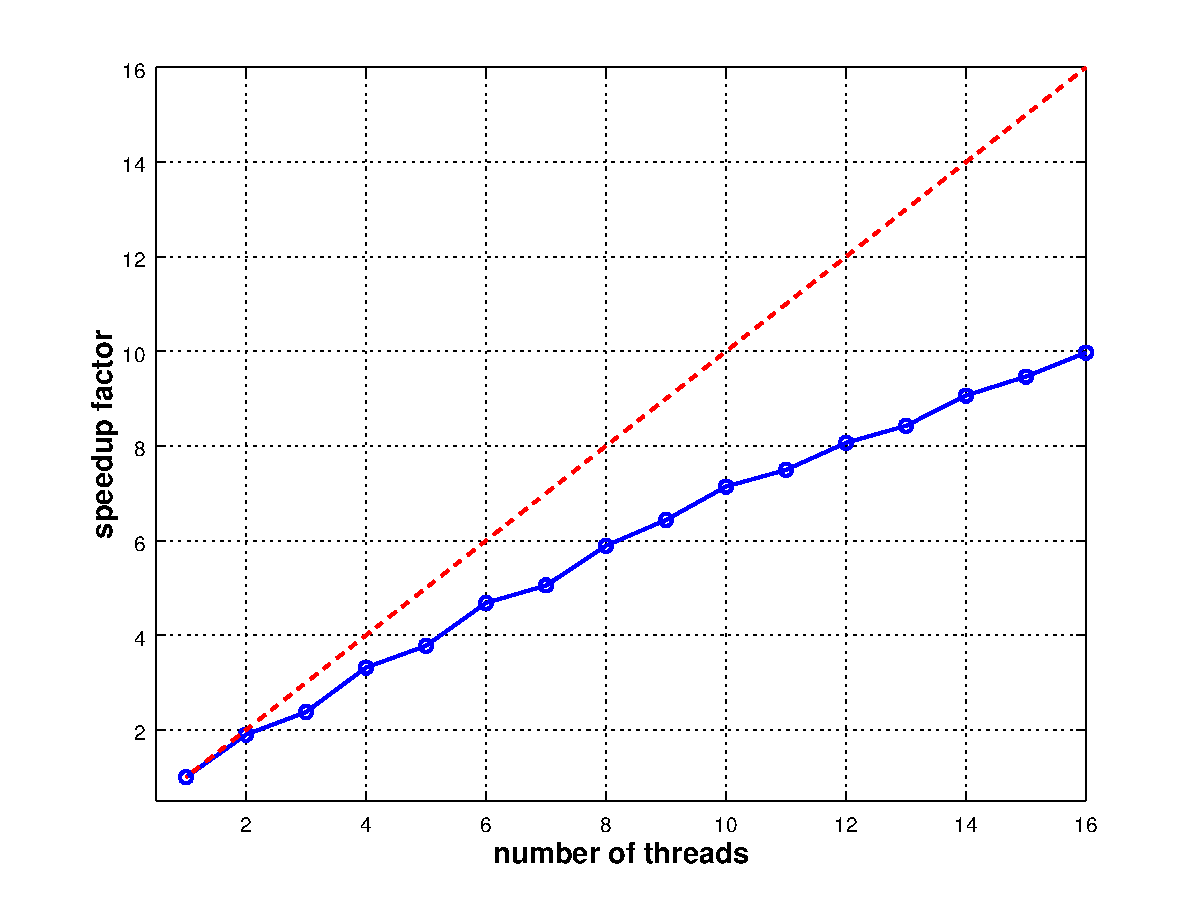
\includegraphics[width=1.1\textwidth]{plot2.pdf}\\
    {(b)}
  \end{minipage}
\end{minipage}
\caption
  {
  Execution characteristics for training a 100 component GMM
  to model a synthetic dataset comprising 1,000,000 samples with 100 dimensions
  using 10 iterations of the {\it k}-means algorithm and 10 iterations of the EM algorithm:
  {\bf (a)}~total time taken depending on the number of threads;
  {\bf (b)}~corresponding speedup factor compared to using one thread (blue line), and idealised linear speedup under the assumption of no overheads and no memory access contention (red dotted line).
  The modelling was done on a machine with dual Intel Xeon E5-2620~v4 CPUs, providing 16 independent processing cores.
  Compilation was done with GCC 5.4 using the following switches: \texttt{-O3 -march=native -fopenmp}.
  }
\label{fig:speedup}
\end{figure*}


% \begin{figure}[!b]
% \hrule
% \vspace{1ex}
% \centering
% \begin{Verbatim}[fontfamily=fvm,fontsize=\footnotesize]
% #include <fstream>
% #include <armadillo>
% 
% using namespace std;
% using namespace arma;
% 
% int main()
%   {
%   // create synthetic data with 100 clusters
%   
%   uword n_gaus = 100;
%   
%   uword d = 100;      // dimensionality
%   uword N = 1000000;  // number of samples (vectors)
%   
%   cout << "generating synthetic data" << endl;
%   
%   mat data(d, N, fill::zeros);
%   
%   mat means(d, n_gaus, fill::zeros);
%   
%   for(uword g=0; g < n_gaus; ++g)
%     {
%     means.col(g) = g + linspace<vec>(1,d,d);
%     }
%   
%   uword i = 0;
%   
%   while(i < N)
%     {
%     for(uword g=0; g < n_gaus; ++g)
%       {
%       if(i < N)  { data.col(i) = means.col(g) + 2*randn<vec>(d); ++i; }
%       }
%     }
%   
%   cout << "modelling data" << endl;
%   
%   wall_clock timer;
%   timer.tic();
%   
%   gmm_diag model;
%   
%   const uword km_iter = 10;
%   const uword em_iter = 10;
%   
%   bool status = model.learn(data, n_gaus, maha_dist, random_subset, km_iter, em_iter, 1e-10, true);
%   
%   if(status == false)  { cout << "learning failed" << endl; }
%   
%   cout << "timer.toc(): " << timer.toc() << endl;
%   
%   return 0;
%   }
% \end{Verbatim}
% \vspace{-1ex}
% \hrule
% \vspace{0.5ex}
% \caption
%   {
%   C++ source code for timing of modelling synthetic data with the {\it gmm\_diag} class.
%   }
% \label{fig:timing_prog}
% \end{figure}
